\
\
\
\
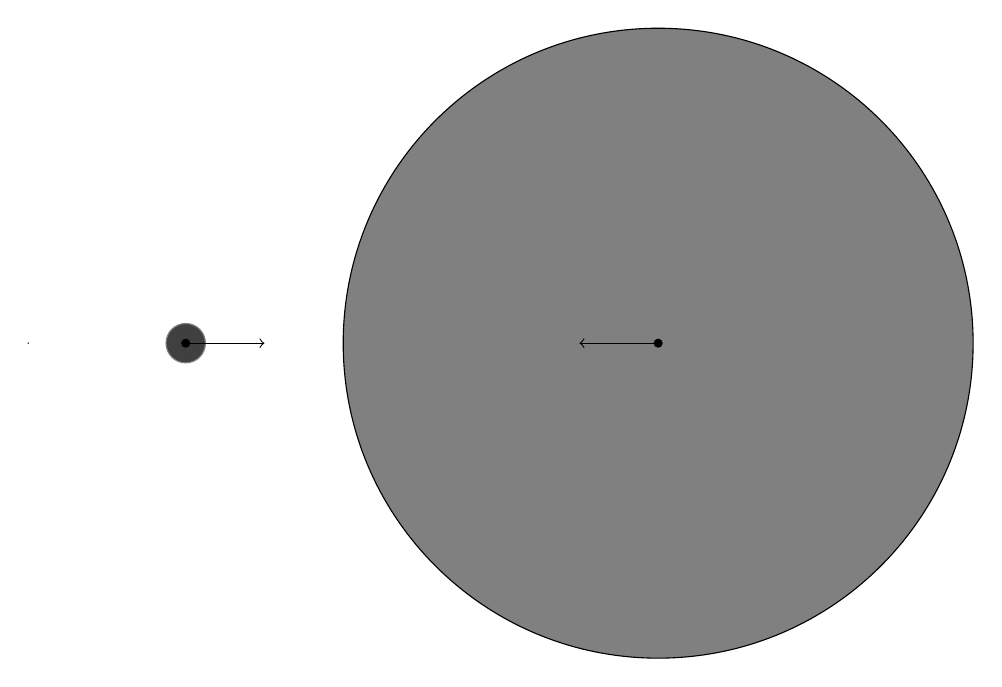
\begin{tikzpicture}
\draw (0,0) circle (0.0001cm);
\filldraw[fill = darkgray, draw= gray] (2,0) circle (0.25cm);
\filldraw[fill = gray, draw = black] (8,0) circle (4cm);
\filldraw (2,0) circle (0.05cm);
\filldraw (8,0) circle (0.05cm);
\draw[->] (2,0) -- (3,0);
\draw[->] (8,0) -- (7,0);
\end{tikzpicture}
\newline
Up until this point we have considered the gravitational potential energy as $mgh$ and the gravitational force as $mg$. However, this definition is only an approximation and only works in the case of an object of small mass that is very close to the surface of the earth. This should not be too much a surprise because it is not as if all objects in the universe are moving towards the earth with acceleration $g$. However, let us try to find out what the gravitational force is just using our intuition. Let us consider the case of two spheres of mass $m_1$ and $m_2$ in a vacuum separated by a distance $R$. It should be obvious that the gravitational force will increase if either one of the masses increases because there Will be more mass for the other mass to pull on. Additionally, it should be intuitive that the farther away the masses are, the smaller the gravitational force will be. We also should think that there will be some constant of proportionality between the factors that we have mentioned so far and the true factor. We will call this constant $G$. I am now going to assert because we can not show it analytically, that the gravitational force varies linearly with the two masses and varies as the inverse squared of the distance between the objects. So we can write that \begin{equation}F_g=\frac{-G m_1 m_2}{r^2}\end{equation} In one sense, we can say that we are now completely done with understanding Newtonian gravitation now that we have this expression. We can say this because we could model all items as being point masses and then plug in a vast number of atoms into our equations and use a computer to find how the atoms will behave. Doing work like this is very prevalent and important, and many numerical methods have been invented with the goal of trying to calculate the solutions to these problems. 
These types of problems quickly get very complicated. Think about it, with three masses; we have already a complex system where the force is constantly changing, and the objects are not going to behave in obvious ways.
\newline
\newline
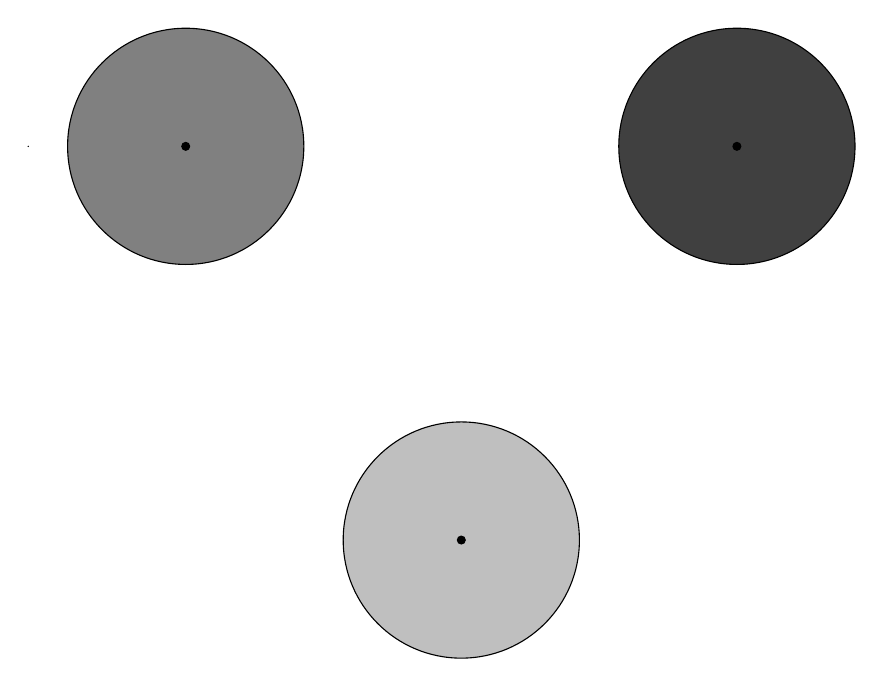
\begin{tikzpicture}
\draw (0,0) circle (0.00001cm);
\filldraw[draw = black, fill = gray] (2,0) circle (1.5cm);
\filldraw[draw = black, fill = darkgray] (9,0) circle (1.5cm);
\filldraw[draw = black, fill = lightgray] (5.5,-5) circle (1.5cm);
\filldraw (2,0) circle (0.05cm);
\filldraw (9,0) circle (0.05cm);
\filldraw (5.5,-5) circle (0.05cm);
\end{tikzpicture}
\begin{center}
(Figure 7.1.1)
\end{center}
\
Even if we use this formula to model an object falling to the earth, we already have to use numerical approximations. Most examples displaying this force will come in later sections, so, for now, we will move on to our discussion of the gravitational potential energy. 
To find the potential energy we are going to find the amount of work it would take to bring two objects from an infinite distance away to their current situation. At first, we imagine there is nothing where the masses are. Now we imagine moving the first mass in. This will not take any work as nothing is pushing or pulling on it to perturb it from its current state. So now we find the work it takes to bring the second mass from infinity to its current state, we will say at a distance $r$ from the other ball. This requires us to do an integral. I will leave this as an exercise to you, but upon completing the integral, we find that the potential energy \begin{equation} U = \frac{-Gm_1m_2}{r}\end{equation} This result is independent of which mass we imagine being brought in first as you can see when doing the calculation. We can use this concept of gravitational potential energy when discussing the motion of objects as they orbit around in space. 